% Options for packages loaded elsewhere
\PassOptionsToPackage{unicode}{hyperref}
\PassOptionsToPackage{hyphens}{url}
\PassOptionsToPackage{dvipsnames,svgnames,x11names}{xcolor}
%
\documentclass[
  letterpaper,
  DIV=11,
  numbers=noendperiod,
  oneside]{scrartcl}

\usepackage{amsmath,amssymb}
\usepackage{iftex}
\ifPDFTeX
  \usepackage[T1]{fontenc}
  \usepackage[utf8]{inputenc}
  \usepackage{textcomp} % provide euro and other symbols
\else % if luatex or xetex
  \usepackage{unicode-math}
  \defaultfontfeatures{Scale=MatchLowercase}
  \defaultfontfeatures[\rmfamily]{Ligatures=TeX,Scale=1}
\fi
\usepackage{lmodern}
\ifPDFTeX\else  
    % xetex/luatex font selection
\fi
% Use upquote if available, for straight quotes in verbatim environments
\IfFileExists{upquote.sty}{\usepackage{upquote}}{}
\IfFileExists{microtype.sty}{% use microtype if available
  \usepackage[]{microtype}
  \UseMicrotypeSet[protrusion]{basicmath} % disable protrusion for tt fonts
}{}
\makeatletter
\@ifundefined{KOMAClassName}{% if non-KOMA class
  \IfFileExists{parskip.sty}{%
    \usepackage{parskip}
  }{% else
    \setlength{\parindent}{0pt}
    \setlength{\parskip}{6pt plus 2pt minus 1pt}}
}{% if KOMA class
  \KOMAoptions{parskip=half}}
\makeatother
\usepackage{xcolor}
\usepackage[left=1in,marginparwidth=2.0666666666667in,textwidth=4.1333333333333in,marginparsep=0.3in]{geometry}
\setlength{\emergencystretch}{3em} % prevent overfull lines
\setcounter{secnumdepth}{-\maxdimen} % remove section numbering
% Make \paragraph and \subparagraph free-standing
\ifx\paragraph\undefined\else
  \let\oldparagraph\paragraph
  \renewcommand{\paragraph}[1]{\oldparagraph{#1}\mbox{}}
\fi
\ifx\subparagraph\undefined\else
  \let\oldsubparagraph\subparagraph
  \renewcommand{\subparagraph}[1]{\oldsubparagraph{#1}\mbox{}}
\fi

\usepackage{color}
\usepackage{fancyvrb}
\newcommand{\VerbBar}{|}
\newcommand{\VERB}{\Verb[commandchars=\\\{\}]}
\DefineVerbatimEnvironment{Highlighting}{Verbatim}{commandchars=\\\{\}}
% Add ',fontsize=\small' for more characters per line
\usepackage{framed}
\definecolor{shadecolor}{RGB}{241,243,245}
\newenvironment{Shaded}{\begin{snugshade}}{\end{snugshade}}
\newcommand{\AlertTok}[1]{\textcolor[rgb]{0.68,0.00,0.00}{#1}}
\newcommand{\AnnotationTok}[1]{\textcolor[rgb]{0.37,0.37,0.37}{#1}}
\newcommand{\AttributeTok}[1]{\textcolor[rgb]{0.40,0.45,0.13}{#1}}
\newcommand{\BaseNTok}[1]{\textcolor[rgb]{0.68,0.00,0.00}{#1}}
\newcommand{\BuiltInTok}[1]{\textcolor[rgb]{0.00,0.23,0.31}{#1}}
\newcommand{\CharTok}[1]{\textcolor[rgb]{0.13,0.47,0.30}{#1}}
\newcommand{\CommentTok}[1]{\textcolor[rgb]{0.37,0.37,0.37}{#1}}
\newcommand{\CommentVarTok}[1]{\textcolor[rgb]{0.37,0.37,0.37}{\textit{#1}}}
\newcommand{\ConstantTok}[1]{\textcolor[rgb]{0.56,0.35,0.01}{#1}}
\newcommand{\ControlFlowTok}[1]{\textcolor[rgb]{0.00,0.23,0.31}{#1}}
\newcommand{\DataTypeTok}[1]{\textcolor[rgb]{0.68,0.00,0.00}{#1}}
\newcommand{\DecValTok}[1]{\textcolor[rgb]{0.68,0.00,0.00}{#1}}
\newcommand{\DocumentationTok}[1]{\textcolor[rgb]{0.37,0.37,0.37}{\textit{#1}}}
\newcommand{\ErrorTok}[1]{\textcolor[rgb]{0.68,0.00,0.00}{#1}}
\newcommand{\ExtensionTok}[1]{\textcolor[rgb]{0.00,0.23,0.31}{#1}}
\newcommand{\FloatTok}[1]{\textcolor[rgb]{0.68,0.00,0.00}{#1}}
\newcommand{\FunctionTok}[1]{\textcolor[rgb]{0.28,0.35,0.67}{#1}}
\newcommand{\ImportTok}[1]{\textcolor[rgb]{0.00,0.46,0.62}{#1}}
\newcommand{\InformationTok}[1]{\textcolor[rgb]{0.37,0.37,0.37}{#1}}
\newcommand{\KeywordTok}[1]{\textcolor[rgb]{0.00,0.23,0.31}{#1}}
\newcommand{\NormalTok}[1]{\textcolor[rgb]{0.00,0.23,0.31}{#1}}
\newcommand{\OperatorTok}[1]{\textcolor[rgb]{0.37,0.37,0.37}{#1}}
\newcommand{\OtherTok}[1]{\textcolor[rgb]{0.00,0.23,0.31}{#1}}
\newcommand{\PreprocessorTok}[1]{\textcolor[rgb]{0.68,0.00,0.00}{#1}}
\newcommand{\RegionMarkerTok}[1]{\textcolor[rgb]{0.00,0.23,0.31}{#1}}
\newcommand{\SpecialCharTok}[1]{\textcolor[rgb]{0.37,0.37,0.37}{#1}}
\newcommand{\SpecialStringTok}[1]{\textcolor[rgb]{0.13,0.47,0.30}{#1}}
\newcommand{\StringTok}[1]{\textcolor[rgb]{0.13,0.47,0.30}{#1}}
\newcommand{\VariableTok}[1]{\textcolor[rgb]{0.07,0.07,0.07}{#1}}
\newcommand{\VerbatimStringTok}[1]{\textcolor[rgb]{0.13,0.47,0.30}{#1}}
\newcommand{\WarningTok}[1]{\textcolor[rgb]{0.37,0.37,0.37}{\textit{#1}}}

\providecommand{\tightlist}{%
  \setlength{\itemsep}{0pt}\setlength{\parskip}{0pt}}\usepackage{longtable,booktabs,array}
\usepackage{calc} % for calculating minipage widths
% Correct order of tables after \paragraph or \subparagraph
\usepackage{etoolbox}
\makeatletter
\patchcmd\longtable{\par}{\if@noskipsec\mbox{}\fi\par}{}{}
\makeatother
% Allow footnotes in longtable head/foot
\IfFileExists{footnotehyper.sty}{\usepackage{footnotehyper}}{\usepackage{footnote}}
\makesavenoteenv{longtable}
\usepackage{graphicx}
\makeatletter
\def\maxwidth{\ifdim\Gin@nat@width>\linewidth\linewidth\else\Gin@nat@width\fi}
\def\maxheight{\ifdim\Gin@nat@height>\textheight\textheight\else\Gin@nat@height\fi}
\makeatother
% Scale images if necessary, so that they will not overflow the page
% margins by default, and it is still possible to overwrite the defaults
% using explicit options in \includegraphics[width, height, ...]{}
\setkeys{Gin}{width=\maxwidth,height=\maxheight,keepaspectratio}
% Set default figure placement to htbp
\makeatletter
\def\fps@figure{htbp}
\makeatother

\KOMAoption{captions}{tableheading}
\makeatletter
\makeatother
\makeatletter
\makeatother
\makeatletter
\@ifpackageloaded{caption}{}{\usepackage{caption}}
\AtBeginDocument{%
\ifdefined\contentsname
  \renewcommand*\contentsname{Índice}
\else
  \newcommand\contentsname{Índice}
\fi
\ifdefined\listfigurename
  \renewcommand*\listfigurename{Lista de Figuras}
\else
  \newcommand\listfigurename{Lista de Figuras}
\fi
\ifdefined\listtablename
  \renewcommand*\listtablename{Lista de Tabelas}
\else
  \newcommand\listtablename{Lista de Tabelas}
\fi
\ifdefined\figurename
  \renewcommand*\figurename{Figura}
\else
  \newcommand\figurename{Figura}
\fi
\ifdefined\tablename
  \renewcommand*\tablename{Tabela}
\else
  \newcommand\tablename{Tabela}
\fi
}
\@ifpackageloaded{float}{}{\usepackage{float}}
\floatstyle{ruled}
\@ifundefined{c@chapter}{\newfloat{codelisting}{h}{lop}}{\newfloat{codelisting}{h}{lop}[chapter]}
\floatname{codelisting}{Listagem}
\newcommand*\listoflistings{\listof{codelisting}{Lista de Listagens}}
\makeatother
\makeatletter
\@ifpackageloaded{caption}{}{\usepackage{caption}}
\@ifpackageloaded{subcaption}{}{\usepackage{subcaption}}
\makeatother
\makeatletter
\@ifpackageloaded{tcolorbox}{}{\usepackage[skins,breakable]{tcolorbox}}
\makeatother
\makeatletter
\@ifundefined{shadecolor}{\definecolor{shadecolor}{rgb}{.97, .97, .97}}
\makeatother
\makeatletter
\makeatother
\makeatletter
\@ifpackageloaded{sidenotes}{}{\usepackage{sidenotes}}
\@ifpackageloaded{marginnote}{}{\usepackage{marginnote}}
\makeatother
\makeatletter
\makeatother
\ifLuaTeX
\usepackage[bidi=basic]{babel}
\else
\usepackage[bidi=default]{babel}
\fi
\babelprovide[main,import]{portuguese}
% get rid of language-specific shorthands (see #6817):
\let\LanguageShortHands\languageshorthands
\def\languageshorthands#1{}
\ifLuaTeX
  \usepackage{selnolig}  % disable illegal ligatures
\fi
\IfFileExists{bookmark.sty}{\usepackage{bookmark}}{\usepackage{hyperref}}
\IfFileExists{xurl.sty}{\usepackage{xurl}}{} % add URL line breaks if available
\urlstyle{same} % disable monospaced font for URLs
\hypersetup{
  pdftitle={Suport Vector Regression Machine - SVRM},
  pdfauthor={Prof.~Dr.~Pedro Rafael D. Marinho},
  pdflang={pt},
  colorlinks=true,
  linkcolor={blue},
  filecolor={Maroon},
  citecolor={Blue},
  urlcolor={Blue},
  pdfcreator={LaTeX via pandoc}}

\title{Suport Vector Regression Machine - SVRM}
\usepackage{etoolbox}
\makeatletter
\providecommand{\subtitle}[1]{% add subtitle to \maketitle
  \apptocmd{\@title}{\par {\large #1 \par}}{}{}
}
\makeatother
\subtitle{Comparando com outros modelos}
\author{Prof.~Dr.~Pedro Rafael D. Marinho}
\date{2023-07-25}

\begin{document}
\maketitle
\ifdefined\Shaded\renewenvironment{Shaded}{\begin{tcolorbox}[frame hidden, borderline west={3pt}{0pt}{shadecolor}, boxrule=0pt, enhanced, sharp corners, breakable, interior hidden]}{\end{tcolorbox}}\fi

\hypertarget{carregando-bibliotecas-necessuxe1rias}{%
\subsection{Carregando bibliotecas
necessárias}\label{carregando-bibliotecas-necessuxe1rias}}

\begin{Shaded}
\begin{Highlighting}[]
\InformationTok{\textasciigrave{}\textasciigrave{}\textasciigrave{}\{r\}}
\FunctionTok{library}\NormalTok{(tidymodels)}
\InformationTok{\textasciigrave{}\textasciigrave{}\textasciigrave{}}
\end{Highlighting}
\end{Shaded}

\begin{verbatim}
-- Attaching packages -------------------------------------- tidymodels 1.1.0 --
\end{verbatim}

\begin{verbatim}
v broom        1.0.5     v recipes      1.0.6
v dials        1.2.0     v rsample      1.1.1
v dplyr        1.1.2     v tibble       3.2.1
v ggplot2      3.4.2     v tidyr        1.3.0
v infer        1.0.4     v tune         1.1.1
v modeldata    1.1.0     v workflows    1.1.3
v parsnip      1.1.0     v workflowsets 1.0.1
v purrr        1.0.1     v yardstick    1.2.0
\end{verbatim}

\begin{verbatim}
-- Conflicts ----------------------------------------- tidymodels_conflicts() --
x purrr::discard() masks scales::discard()
x dplyr::filter()  masks stats::filter()
x dplyr::lag()     masks stats::lag()
x recipes::step()  masks stats::step()
* Dig deeper into tidy modeling with R at https://www.tmwr.org
\end{verbatim}

\begin{Shaded}
\begin{Highlighting}[]
\InformationTok{\textasciigrave{}\textasciigrave{}\textasciigrave{}\{r\}}
\FunctionTok{library}\NormalTok{(tidyverse)}
\InformationTok{\textasciigrave{}\textasciigrave{}\textasciigrave{}}
\end{Highlighting}
\end{Shaded}

\begin{verbatim}
-- Attaching core tidyverse packages ------------------------ tidyverse 2.0.0 --
v forcats   1.0.0     v readr     2.1.4
v lubridate 1.9.2     v stringr   1.5.0
\end{verbatim}

\begin{verbatim}
-- Conflicts ------------------------------------------ tidyverse_conflicts() --
x readr::col_factor() masks scales::col_factor()
x purrr::discard()    masks scales::discard()
x dplyr::filter()     masks stats::filter()
x stringr::fixed()    masks recipes::fixed()
x dplyr::lag()        masks stats::lag()
x readr::spec()       masks yardstick::spec()
i Use the conflicted package (<http://conflicted.r-lib.org/>) to force all conflicts to become errors
\end{verbatim}

\begin{Shaded}
\begin{Highlighting}[]
\InformationTok{\textasciigrave{}\textasciigrave{}\textasciigrave{}\{r\}}
\FunctionTok{library}\NormalTok{(GGally)}
\InformationTok{\textasciigrave{}\textasciigrave{}\textasciigrave{}}
\end{Highlighting}
\end{Shaded}

\begin{verbatim}
Registered S3 method overwritten by 'GGally':
  method from   
  +.gg   ggplot2
\end{verbatim}

\begin{Shaded}
\begin{Highlighting}[]
\InformationTok{\textasciigrave{}\textasciigrave{}\textasciigrave{}\{r\}}
\FunctionTok{library}\NormalTok{(skimr)}

\CommentTok{\# Resolvendo possíveis conflitos entre o tidymodels e outras bibliotecas}
\NormalTok{tidymodels}\SpecialCharTok{::}\FunctionTok{tidymodels\_prefer}\NormalTok{()}
\InformationTok{\textasciigrave{}\textasciigrave{}\textasciigrave{}}
\end{Highlighting}
\end{Shaded}

\hypertarget{importando-a-base-de-dados}{%
\subsection{Importando a base de
dados}\label{importando-a-base-de-dados}}

Utilizando os dados de vinho vermelho🍷, disponíveis
\href{https://www.kaggle.com/datasets/uciml/red-wine-quality-cortez-et-al-2009}{aqui},
faça uma pequena análise exploratória dos dados. No
\href{https://www.kaggle.com/datasets/uciml/red-wine-quality-cortez-et-al-2009}{link}
do Kaggle você consegue uma explicação sobre o que significa cada uma
das variáveis.

Os dados, no meu caso, estão no diretório
\texttt{"../dados/winequality-red.csv"}. Você deverá alterar o
\emph{path} para o diretório encontra-se a base que deverá ser obtida no
link acima.

\begin{Shaded}
\begin{Highlighting}[]
\InformationTok{\textasciigrave{}\textasciigrave{}\textasciigrave{}\{r\}}
\NormalTok{dados }\OtherTok{\textless{}{-}}\NormalTok{ readr}\SpecialCharTok{::}\FunctionTok{read\_csv}\NormalTok{(}\AttributeTok{file =} \StringTok{"../dados/winequality{-}red.csv"}\NormalTok{)}
\InformationTok{\textasciigrave{}\textasciigrave{}\textasciigrave{}}
\end{Highlighting}
\end{Shaded}

\begin{verbatim}
Rows: 1599 Columns: 12
-- Column specification --------------------------------------------------------
Delimiter: ","
dbl (12): fixed acidity, volatile acidity, citric acid, residual sugar, chlo...

i Use `spec()` to retrieve the full column specification for this data.
i Specify the column types or set `show_col_types = FALSE` to quiet this message.
\end{verbatim}

\hypertarget{uma-explorauxe7uxe3o-ruxe1pida-dos-dados}{%
\subsection{Uma exploração rápida dos
dados}\label{uma-explorauxe7uxe3o-ruxe1pida-dos-dados}}

É sempre importante olhar os dados antes de tentar modelar. Uma análise
exploratória sempre será útil para identificarmos possíveis
inconsistências.

\begin{Shaded}
\begin{Highlighting}[]
\InformationTok{\textasciigrave{}\textasciigrave{}\textasciigrave{}\{r\}}
\NormalTok{visdat}\SpecialCharTok{::}\FunctionTok{vis\_dat}\NormalTok{(dados)}
\InformationTok{\textasciigrave{}\textasciigrave{}\textasciigrave{}}
\end{Highlighting}
\end{Shaded}

\begin{figure}[H]

{\centering 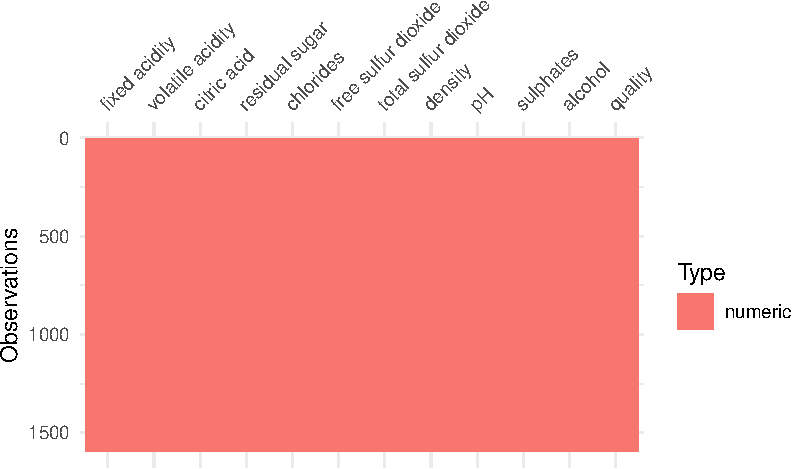
\includegraphics{tufte_svm_regressao_files/figure-pdf/unnamed-chunk-3-1.pdf}

}

\end{figure}

O gráfico acima mostra que temos uma base de dados sem informações
faltantes e todas as \emph{features} presentes na base são numéricas. É
uma situação confortável, haja vista que, aqui, não precisaremos nos
preocupar com imputação de dados faltantes.

Um resumo dos dados poderá ser obtido utilizando a função
\texttt{glimpse} do pacote \textbf{dplyr} que é carregado com a
biblioteca \textbf{tidyverse} de R.

\begin{Shaded}
\begin{Highlighting}[]
\InformationTok{\textasciigrave{}\textasciigrave{}\textasciigrave{}\{r\}}
\NormalTok{dados }\SpecialCharTok{|\textgreater{}} 
\NormalTok{  dplyr}\SpecialCharTok{::}\FunctionTok{glimpse}\NormalTok{()}
\InformationTok{\textasciigrave{}\textasciigrave{}\textasciigrave{}}
\end{Highlighting}
\end{Shaded}

\begin{verbatim}
Rows: 1,599
Columns: 12
$ `fixed acidity`        <dbl> 7.4, 7.8, 7.8, 11.2, 7.4, 7.4, 7.9, 7.3, 7.8, 7~
$ `volatile acidity`     <dbl> 0.700, 0.880, 0.760, 0.280, 0.700, 0.660, 0.600~
$ `citric acid`          <dbl> 0.00, 0.00, 0.04, 0.56, 0.00, 0.00, 0.06, 0.00,~
$ `residual sugar`       <dbl> 1.9, 2.6, 2.3, 1.9, 1.9, 1.8, 1.6, 1.2, 2.0, 6.~
$ chlorides              <dbl> 0.076, 0.098, 0.092, 0.075, 0.076, 0.075, 0.069~
$ `free sulfur dioxide`  <dbl> 11, 25, 15, 17, 11, 13, 15, 15, 9, 17, 15, 17, ~
$ `total sulfur dioxide` <dbl> 34, 67, 54, 60, 34, 40, 59, 21, 18, 102, 65, 10~
$ density                <dbl> 0.9978, 0.9968, 0.9970, 0.9980, 0.9978, 0.9978,~
$ pH                     <dbl> 3.51, 3.20, 3.26, 3.16, 3.51, 3.51, 3.30, 3.39,~
$ sulphates              <dbl> 0.56, 0.68, 0.65, 0.58, 0.56, 0.56, 0.46, 0.47,~
$ alcohol                <dbl> 9.4, 9.8, 9.8, 9.8, 9.4, 9.4, 9.4, 10.0, 9.5, 1~
$ quality                <dbl> 5, 5, 5, 6, 5, 5, 5, 7, 7, 5, 5, 5, 5, 5, 5, 5,~
\end{verbatim}

É possível todas as correlações entre todas as variáveis da base, com a
função \texttt{data\_vis\_cor}. Um gráfico útil com as correlações
poderá ser obtido usando a função \texttt{vis\_cor}, conforme abaixo:

\begin{Shaded}
\begin{Highlighting}[]
\InformationTok{\textasciigrave{}\textasciigrave{}\textasciigrave{}\{r\}}
\NormalTok{visdat}\SpecialCharTok{::}\FunctionTok{data\_vis\_cor}\NormalTok{(dados)}
\NormalTok{visdat}\SpecialCharTok{::}\FunctionTok{vis\_cor}\NormalTok{(dados)}
\InformationTok{\textasciigrave{}\textasciigrave{}\textasciigrave{}}
\end{Highlighting}
\end{Shaded}

\begin{verbatim}
# A tibble: 144 x 3
   row_1         row_2                  value
   <chr>         <chr>                  <dbl>
 1 fixed acidity fixed acidity         1     
 2 fixed acidity volatile acidity     -0.256 
 3 fixed acidity citric acid           0.672 
 4 fixed acidity residual sugar        0.115 
 5 fixed acidity chlorides             0.0937
 6 fixed acidity free sulfur dioxide  -0.154 
 7 fixed acidity total sulfur dioxide -0.113 
 8 fixed acidity density               0.668 
 9 fixed acidity pH                   -0.683 
10 fixed acidity sulphates             0.183 
# i 134 more rows
\end{verbatim}

\begin{figure}[H]

{\centering 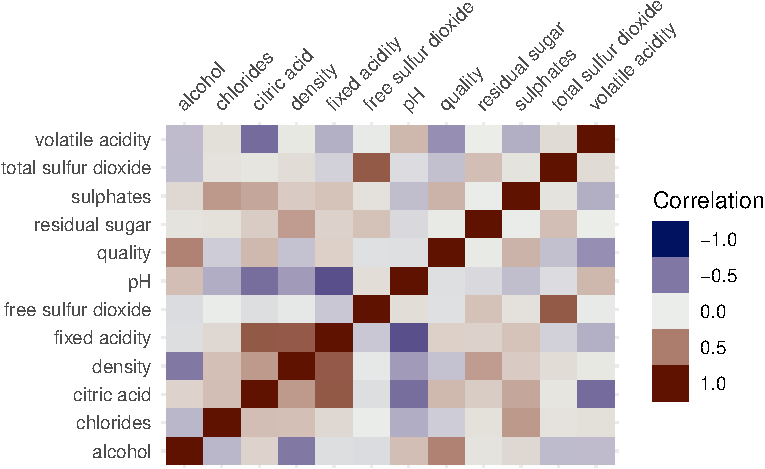
\includegraphics{tufte_svm_regressao_files/figure-pdf/unnamed-chunk-5-1.pdf}

}

\end{figure}

Um gráfico de scatterplot para as variáveis numéricas poderá ser útil.
Você poderá fazer isso, usando a função \texttt{ggcatmat} do pacote
\href{https://ggobi.github.io/ggally/index.html}{GGally}.

\begin{Shaded}
\begin{Highlighting}[]
\InformationTok{\textasciigrave{}\textasciigrave{}\textasciigrave{}\{r\}}
\NormalTok{dados }\SpecialCharTok{|\textgreater{}} 
\NormalTok{  GGally}\SpecialCharTok{::}\FunctionTok{ggscatmat}\NormalTok{()}
\InformationTok{\textasciigrave{}\textasciigrave{}\textasciigrave{}}
\end{Highlighting}
\end{Shaded}

\begin{verbatim}
Warning: The dot-dot notation (`..scaled..`) was deprecated in ggplot2 3.4.0.
i Please use `after_stat(scaled)` instead.
i The deprecated feature was likely used in the GGally package.
  Please report the issue at <https://github.com/ggobi/ggally/issues>.
\end{verbatim}

\begin{figure}[H]

{\centering 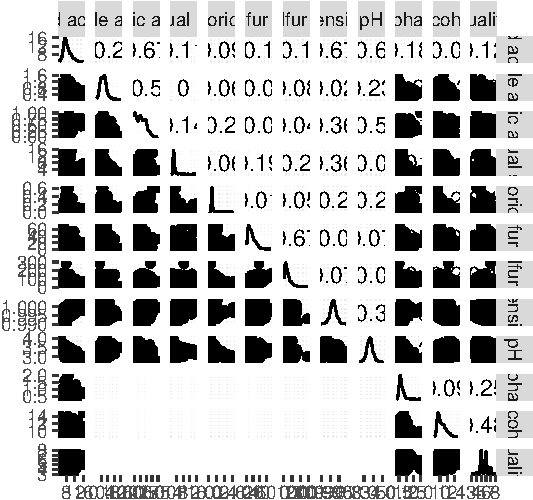
\includegraphics{tufte_svm_regressao_files/figure-pdf/unnamed-chunk-6-1.pdf}

}

\end{figure}

As bibliotecas \textbf{GGally} e \textbf{skimr} também possuem funções
úteis que podem nos auxiliar no processo de exploração dos dados.

\begin{Shaded}
\begin{Highlighting}[]
\InformationTok{\textasciigrave{}\textasciigrave{}\textasciigrave{}\{r\}}
\NormalTok{dados }\SpecialCharTok{|\textgreater{}} 
\NormalTok{  GGally}\SpecialCharTok{::}\FunctionTok{ggpairs}\NormalTok{()}

\NormalTok{dados }\SpecialCharTok{|\textgreater{}} 
\NormalTok{  skimr}\SpecialCharTok{::}\FunctionTok{skim}\NormalTok{()}
\InformationTok{\textasciigrave{}\textasciigrave{}\textasciigrave{}}
\end{Highlighting}
\end{Shaded}

\begin{longtable}[]{@{}ll@{}}
\caption{Data summary}\tabularnewline
\toprule\noalign{}
\endfirsthead
\endhead
\bottomrule\noalign{}
\endlastfoot
Name & dados \\
Number of rows & 1599 \\
Number of columns & 12 \\
\_\_\_\_\_\_\_\_\_\_\_\_\_\_\_\_\_\_\_\_\_\_\_ & \\
Column type frequency: & \\
numeric & 12 \\
\_\_\_\_\_\_\_\_\_\_\_\_\_\_\_\_\_\_\_\_\_\_\_\_ & \\
Group variables & None \\
\end{longtable}

\textbf{Variable type: numeric}

\begin{longtable}[]{@{}
  >{\raggedright\arraybackslash}p{(\columnwidth - 20\tabcolsep) * \real{0.2258}}
  >{\raggedleft\arraybackslash}p{(\columnwidth - 20\tabcolsep) * \real{0.1075}}
  >{\raggedleft\arraybackslash}p{(\columnwidth - 20\tabcolsep) * \real{0.1505}}
  >{\raggedleft\arraybackslash}p{(\columnwidth - 20\tabcolsep) * \real{0.0645}}
  >{\raggedleft\arraybackslash}p{(\columnwidth - 20\tabcolsep) * \real{0.0645}}
  >{\raggedleft\arraybackslash}p{(\columnwidth - 20\tabcolsep) * \real{0.0538}}
  >{\raggedleft\arraybackslash}p{(\columnwidth - 20\tabcolsep) * \real{0.0645}}
  >{\raggedleft\arraybackslash}p{(\columnwidth - 20\tabcolsep) * \real{0.0645}}
  >{\raggedleft\arraybackslash}p{(\columnwidth - 20\tabcolsep) * \real{0.0645}}
  >{\raggedleft\arraybackslash}p{(\columnwidth - 20\tabcolsep) * \real{0.0753}}
  >{\raggedright\arraybackslash}p{(\columnwidth - 20\tabcolsep) * \real{0.0645}}@{}}
\toprule\noalign{}
\begin{minipage}[b]{\linewidth}\raggedright
skim\_variable
\end{minipage} & \begin{minipage}[b]{\linewidth}\raggedleft
n\_missing
\end{minipage} & \begin{minipage}[b]{\linewidth}\raggedleft
complete\_rate
\end{minipage} & \begin{minipage}[b]{\linewidth}\raggedleft
mean
\end{minipage} & \begin{minipage}[b]{\linewidth}\raggedleft
sd
\end{minipage} & \begin{minipage}[b]{\linewidth}\raggedleft
p0
\end{minipage} & \begin{minipage}[b]{\linewidth}\raggedleft
p25
\end{minipage} & \begin{minipage}[b]{\linewidth}\raggedleft
p50
\end{minipage} & \begin{minipage}[b]{\linewidth}\raggedleft
p75
\end{minipage} & \begin{minipage}[b]{\linewidth}\raggedleft
p100
\end{minipage} & \begin{minipage}[b]{\linewidth}\raggedright
hist
\end{minipage} \\
\midrule\noalign{}
\endhead
\bottomrule\noalign{}
\endlastfoot
fixed acidity & 0 & 1 & 8.32 & 1.74 & 4.60 & 7.10 & 7.90 & 9.20 & 15.90
& ▂▇▂▁▁ \\
volatile acidity & 0 & 1 & 0.53 & 0.18 & 0.12 & 0.39 & 0.52 & 0.64 &
1.58 & ▅▇▂▁▁ \\
citric acid & 0 & 1 & 0.27 & 0.19 & 0.00 & 0.09 & 0.26 & 0.42 & 1.00 &
▇▆▅▁▁ \\
residual sugar & 0 & 1 & 2.54 & 1.41 & 0.90 & 1.90 & 2.20 & 2.60 & 15.50
& ▇▁▁▁▁ \\
chlorides & 0 & 1 & 0.09 & 0.05 & 0.01 & 0.07 & 0.08 & 0.09 & 0.61 &
▇▁▁▁▁ \\
free sulfur dioxide & 0 & 1 & 15.87 & 10.46 & 1.00 & 7.00 & 14.00 &
21.00 & 72.00 & ▇▅▁▁▁ \\
total sulfur dioxide & 0 & 1 & 46.47 & 32.90 & 6.00 & 22.00 & 38.00 &
62.00 & 289.00 & ▇▂▁▁▁ \\
density & 0 & 1 & 1.00 & 0.00 & 0.99 & 1.00 & 1.00 & 1.00 & 1.00 &
▁▃▇▂▁ \\
pH & 0 & 1 & 3.31 & 0.15 & 2.74 & 3.21 & 3.31 & 3.40 & 4.01 & ▁▅▇▂▁ \\
sulphates & 0 & 1 & 0.66 & 0.17 & 0.33 & 0.55 & 0.62 & 0.73 & 2.00 &
▇▅▁▁▁ \\
alcohol & 0 & 1 & 10.42 & 1.07 & 8.40 & 9.50 & 10.20 & 11.10 & 14.90 &
▇▇▃▁▁ \\
quality & 0 & 1 & 5.64 & 0.81 & 3.00 & 5.00 & 6.00 & 6.00 & 8.00 &
▁▇▇▂▁ \\
\end{longtable}

\begin{figure}[H]

{\centering 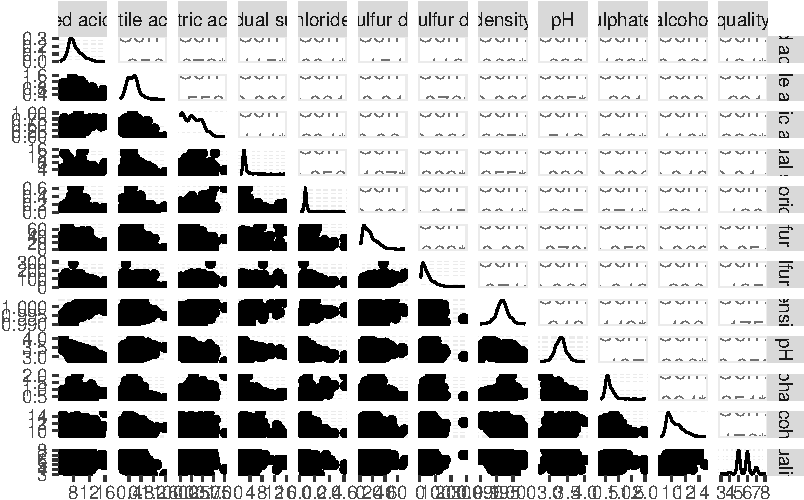
\includegraphics{tufte_svm_regressao_files/figure-pdf/unnamed-chunk-7-1.pdf}

}

\end{figure}

\hypertarget{construindo-os-workflows-dos-modelos}{%
\subsection{Construindo os workflows dos
modelos}\label{construindo-os-workflows-dos-modelos}}

Iremos comparar os modelos de regressão linar utilizando \emph{elastic
net}, com o método \(k\)NN e \emph{suport vector regression machine} -
SVRM. Buscaremos pelo melhor modelo de cada uma das metodologias
consideradas. Posteriormente iremos escolher o melhor modelo entre os
melhores de cada uma das classes. A ideia é escolher o melhor modelo que
consiga prever melhor a qualidade do vinho, i.e., prever a variável
\texttt{quality}.

\hypertarget{divisuxe3o-dos-dados}{%
\subsubsection{Divisão dos dados}\label{divisuxe3o-dos-dados}}

Aqui usaremos as funções \texttt{initial\_split}, \texttt{training} e
\texttt{testing} para realizar o método \emph{hold-out} (divisão inicial
dos dados) em treino e teste. Vamos considerar \(80\%\) para treino e
\(20\%\) para teste. A função \texttt{initial\_split} irá realizar a
divisão, porém, as funções \texttt{training} e \texttt{testing} são
responsáveis para obtermos as tibbles da base de treino e teste,
respectivamente.

Aqui, os dados está sendo estratificado pelo \emph{label}, i.e., pela
variável \texttt{quality} que desejamos prever:

\begin{Shaded}
\begin{Highlighting}[]
\InformationTok{\textasciigrave{}\textasciigrave{}\textasciigrave{}\{r\}}
\FunctionTok{set.seed}\NormalTok{(}\DecValTok{0}\NormalTok{) }\CommentTok{\# Fixando uma semente}
\NormalTok{divisao\_inicial }\OtherTok{\textless{}{-}}\NormalTok{ rsample}\SpecialCharTok{::}\FunctionTok{initial\_split}\NormalTok{(dados, }\AttributeTok{prop =} \FloatTok{0.8}\NormalTok{, }\AttributeTok{strata =} \StringTok{"quality"}\NormalTok{)}
\NormalTok{treinamento }\OtherTok{\textless{}{-}}\NormalTok{ rsample}\SpecialCharTok{::}\FunctionTok{training}\NormalTok{(divisao\_inicial) }\CommentTok{\# Conjunto de treinamento}
\NormalTok{teste }\OtherTok{\textless{}{-}}\NormalTok{ rsample}\SpecialCharTok{::}\FunctionTok{testing}\NormalTok{(divisao\_inicial) }\CommentTok{\# Conjunto de teste}
\InformationTok{\textasciigrave{}\textasciigrave{}\textasciigrave{}}
\end{Highlighting}
\end{Shaded}

\hypertarget{tratamento-dos-dados-pruxe9-processamento}{%
\subsubsection{Tratamento dos dados
(pré-processamento)}\label{tratamento-dos-dados-pruxe9-processamento}}

Apesar de não haver muito o que fazer nos dados que estamos utilizando
nesse exemplo, em que nosso objetivo aqui é ter uma análise explicativa
de como comparar modelos usando o
\href{https://www.tidymodels.org/}{tidymodels}, iremos utilizar a
biblioteca \href{https://recipes.tidymodels.org/}{recipes}. Os dados
contém apenas variáveis numéricas com todas informações presentes,
tornando o problema um pouco mais simples.

\textbf{Na receita, iremos colocar as seguintes etapas}:

\begin{enumerate}
\def\labelenumi{\arabic{enumi}.}
\tightlist
\item
  Tomaremos o logarítmo de todas as variáveis peditoras
  (\emph{features});
\item
  Remover variáveis preditoras (\emph{features}) que eventualmente estão
  altamente correlacionadas (usando a função \texttt{step\_corr});
\item
  Remover variáveis que possam ter variância próxima à zero, i.e., que
  sejam aproximadamente constantes (usando \texttt{step\_zv});
\item
  Normalizar os dados utilizando a função \texttt{step\_normalize}.
\end{enumerate}

Para que iremos remover variáveis altamente correlacionadas apenas nas
variáveis preditoras, utilizamos a função \texttt{all\_predictors} como
argumentod a função \texttt{step\_corr}. Já no passo de normalização dos
dados, quando consideramos todas as variáveis numéricas, passamos para a
função \texttt{step\_normalize} a função \texttt{all\_numeric} que
especifica que deverá ser normalizado todas as variáveis numéricas. Na
verdade, a normalização se dá em todas as variáveis numéricas, e
portanto, esse argumento poderia ser omitido. Além disso, toda nossa
base é formada por variáveis numéricas, o que torna redundante o uso,
mas irei deixar explícito que todas as variáveis numéricas estão sendo
normalizadas.

\begin{Shaded}
\begin{Highlighting}[]
\InformationTok{\textasciigrave{}\textasciigrave{}\textasciigrave{}\{r\}}
\NormalTok{receita\_1 }\OtherTok{\textless{}{-}} 
\NormalTok{  treinamento }\SpecialCharTok{|\textgreater{}} 
    \FunctionTok{recipe}\NormalTok{(}\AttributeTok{formula =}\NormalTok{ quality }\SpecialCharTok{\textasciitilde{}}\NormalTok{ .) }\SpecialCharTok{|\textgreater{}}
    \FunctionTok{step\_YeoJohnson}\NormalTok{(}\FunctionTok{all\_predictors}\NormalTok{()) }\SpecialCharTok{|\textgreater{}}
    \FunctionTok{step\_normalize}\NormalTok{(}\FunctionTok{all\_predictors}\NormalTok{()) }\SpecialCharTok{|\textgreater{}}
    \FunctionTok{step\_zv}\NormalTok{(}\FunctionTok{all\_predictors}\NormalTok{()) }\SpecialCharTok{|\textgreater{}}
    \FunctionTok{step\_corr}\NormalTok{(}\FunctionTok{all\_predictors}\NormalTok{())}

\NormalTok{receita\_2 }\OtherTok{\textless{}{-}} 
\NormalTok{  treinamento }\SpecialCharTok{|\textgreater{}} 
    \FunctionTok{recipe}\NormalTok{(}\AttributeTok{formula =}\NormalTok{ quality }\SpecialCharTok{\textasciitilde{}}\NormalTok{ .) }\SpecialCharTok{|\textgreater{}}
    \FunctionTok{step\_YeoJohnson}\NormalTok{(}\FunctionTok{all\_predictors}\NormalTok{()) }\SpecialCharTok{|\textgreater{}}
    \FunctionTok{step\_normalize}\NormalTok{(}\FunctionTok{all\_predictors}\NormalTok{())}
\InformationTok{\textasciigrave{}\textasciigrave{}\textasciigrave{}}
\end{Highlighting}
\end{Shaded}

\textbf{Como fazemos para observar se nosso pré-processamento
funcionou?}

\includegraphics{../gifs/hum.gif}

Fácil, assim:

\begin{Shaded}
\begin{Highlighting}[]
\InformationTok{\textasciigrave{}\textasciigrave{}\textasciigrave{}\{r\}}
\NormalTok{receita\_1 }\SpecialCharTok{|\textgreater{}} 
  \FunctionTok{prep}\NormalTok{() }\SpecialCharTok{|\textgreater{}} 
  \FunctionTok{juice}\NormalTok{()}
\InformationTok{\textasciigrave{}\textasciigrave{}\textasciigrave{}}
\end{Highlighting}
\end{Shaded}

\begin{verbatim}
# A tibble: 1,278 x 12
   `fixed acidity` `volatile acidity` `citric acid` `residual sugar` chlorides
             <dbl>              <dbl>         <dbl>            <dbl>     <dbl>
 1         -0.446              1.00          -1.52            -0.602   -0.245 
 2         -0.162              1.77          -1.52             0.559    0.198 
 3         -0.162              1.28          -1.25             0.154    0.0774
 4         -0.446              1.00          -1.52            -0.602   -0.245 
 5         -0.446              0.813         -1.52            -0.845   -0.265 
 6         -0.0949             0.508         -1.12            -1.42    -0.386 
 7         -0.373             -0.0496         0.527            2.10    -0.346 
 8         -1.01               0.402         -0.994           -0.845    0.178 
 9         -0.373             -0.0496         0.527            2.10    -0.346 
10         -0.162              0.560          0.186           -1.42     0.521 
# i 1,268 more rows
# i 7 more variables: `free sulfur dioxide` <dbl>,
#   `total sulfur dioxide` <dbl>, density <dbl>, pH <dbl>, sulphates <dbl>,
#   alcohol <dbl>, quality <dbl>
\end{verbatim}

A função \texttt{prep} estima uma receita de pré-processamento. Algumas
funções \texttt{step\_*} pode conter parâmetros que devem ser estimados.
Inclusive, poderemos tunar esses parâmetros com a função \texttt{tune}
do pacote \href{https://tune.tidymodels.org/}{tune}. Por exemplo, se
tivessemos interesse em interpolar uma \emph{feature} usando a função
\texttt{step\_ns}, o argumento \texttt{deg\_free} que refere-se ao grau
do polinômio poderia ser ``tunado''.

Todas as etapas de pré-processamento são estimadas em cima do conjunto
de dados de treinamento. Por exemplo, na etapa em que realiza-se a
normalização dos dados, a média a variância dos dados são estimadas uma
única vez na base de dados completa, e sempre que essa refeita for
aplicada a novos dados, será utilizado essa mesma média e variância, ou
seja, \textbf{não será recalculada com base no novo conjunto de dados}.

Poderíamos utilizar a função \texttt{bake} ao invés da \texttt{juice}. A
diferença de uma para a outra é que a função \texttt{bake} utiliza uma
receita já estimada com \texttt{prep} e poderá ser aplicada à novos
dados. Já a \texttt{juice} retorna a tibble com a receita preparada para
o conjunto de dados de treinamento, ou ao conjunto de dados ao qual uma
receita foi preparada com \texttt{prep}. Usando \texttt{bake} para o
conjunto de dados de treinamento, poderíamos fazer:

\begin{Shaded}
\begin{Highlighting}[]
\InformationTok{\textasciigrave{}\textasciigrave{}\textasciigrave{}\{r\}}
\NormalTok{receita\_1 }\SpecialCharTok{|\textgreater{}} 
  \FunctionTok{prep}\NormalTok{() }\SpecialCharTok{|\textgreater{}} 
  \FunctionTok{bake}\NormalTok{(}\AttributeTok{new\_data =}\NormalTok{ treinamento)}
\InformationTok{\textasciigrave{}\textasciigrave{}\textasciigrave{}}
\end{Highlighting}
\end{Shaded}

\begin{verbatim}
# A tibble: 1,278 x 12
   `fixed acidity` `volatile acidity` `citric acid` `residual sugar` chlorides
             <dbl>              <dbl>         <dbl>            <dbl>     <dbl>
 1         -0.446              1.00          -1.52            -0.602   -0.245 
 2         -0.162              1.77          -1.52             0.559    0.198 
 3         -0.162              1.28          -1.25             0.154    0.0774
 4         -0.446              1.00          -1.52            -0.602   -0.245 
 5         -0.446              0.813         -1.52            -0.845   -0.265 
 6         -0.0949             0.508         -1.12            -1.42    -0.386 
 7         -0.373             -0.0496         0.527            2.10    -0.346 
 8         -1.01               0.402         -0.994           -0.845    0.178 
 9         -0.373             -0.0496         0.527            2.10    -0.346 
10         -0.162              0.560          0.186           -1.42     0.521 
# i 1,268 more rows
# i 7 more variables: `free sulfur dioxide` <dbl>,
#   `total sulfur dioxide` <dbl>, density <dbl>, pH <dbl>, sulphates <dbl>,
#   alcohol <dbl>, quality <dbl>
\end{verbatim}

\hypertarget{definindo-os-modelos}{%
\subsubsection{Definindo os modelos}\label{definindo-os-modelos}}

O código que segue faz a configuração realiza a configuração dos modelos
que serão comparados. O código \texttt{tune::tune()} especifica que o
respectivo parâmetro de sintonização será obtido no processo de
validação cruzada, particularmente, um \emph{grid search}.

\begin{Shaded}
\begin{Highlighting}[]
\InformationTok{\textasciigrave{}\textasciigrave{}\textasciigrave{}\{r\}}
\NormalTok{modelo\_elastic }\OtherTok{\textless{}{-}} 
\NormalTok{  parsnip}\SpecialCharTok{::}\FunctionTok{linear\_reg}\NormalTok{(}\AttributeTok{penalty =}\NormalTok{ tune}\SpecialCharTok{::}\FunctionTok{tune}\NormalTok{(), }\AttributeTok{mixture =}\NormalTok{ tune}\SpecialCharTok{::}\FunctionTok{tune}\NormalTok{()) }\SpecialCharTok{|\textgreater{}} 
\NormalTok{  parsnip}\SpecialCharTok{::}\FunctionTok{set\_mode}\NormalTok{(}\StringTok{"regression"}\NormalTok{) }\SpecialCharTok{|\textgreater{}} 
\NormalTok{  parsnip}\SpecialCharTok{::}\FunctionTok{set\_engine}\NormalTok{(}\StringTok{"glmnet"}\NormalTok{)}

\NormalTok{modelo\_knn }\OtherTok{\textless{}{-}}
\NormalTok{  parsnip}\SpecialCharTok{::}\FunctionTok{nearest\_neighbor}\NormalTok{(}
    \AttributeTok{neighbors =}\NormalTok{ tune}\SpecialCharTok{::}\FunctionTok{tune}\NormalTok{(),}
    \AttributeTok{dist\_power =}\NormalTok{ tune}\SpecialCharTok{::}\FunctionTok{tune}\NormalTok{(), }
    \AttributeTok{weight\_func =} \StringTok{"gaussian"} 
\NormalTok{  ) }\SpecialCharTok{|\textgreater{}} 
\NormalTok{  parsnip}\SpecialCharTok{::}\FunctionTok{set\_mode}\NormalTok{(}\StringTok{"regression"}\NormalTok{) }\SpecialCharTok{|\textgreater{}} 
\NormalTok{  parsnip}\SpecialCharTok{::}\FunctionTok{set\_engine}\NormalTok{(}\StringTok{"kknn"}\NormalTok{)}

\NormalTok{modelo\_svm }\OtherTok{\textless{}{-}} 
\NormalTok{  parsnip}\SpecialCharTok{::}\FunctionTok{svm\_rbf}\NormalTok{(}
    \AttributeTok{cost =}\NormalTok{ tune}\SpecialCharTok{::}\FunctionTok{tune}\NormalTok{(),}
    \AttributeTok{rbf\_sigma =}\NormalTok{ tune}\SpecialCharTok{::}\FunctionTok{tune}\NormalTok{(),}
    \AttributeTok{margin =}\NormalTok{ tune}\SpecialCharTok{::}\FunctionTok{tune}\NormalTok{()}
\NormalTok{  ) }\SpecialCharTok{|\textgreater{}} 
\NormalTok{  parsnip}\SpecialCharTok{::}\FunctionTok{set\_mode}\NormalTok{(}\StringTok{"regression"}\NormalTok{) }\SpecialCharTok{|\textgreater{}} 
\NormalTok{  parsnip}\SpecialCharTok{::}\FunctionTok{set\_engine}\NormalTok{(}\StringTok{"kernlab"}\NormalTok{)}
\InformationTok{\textasciigrave{}\textasciigrave{}\textasciigrave{}}
\end{Highlighting}
\end{Shaded}

\hypertarget{criando-o-conjunto-de-validauxe7uxe3o}{%
\subsubsection{Criando o conjunto de
validação}\label{criando-o-conjunto-de-validauxe7uxe3o}}

Uma vez que temos a divisão dos dados em conjunto de treinamento e
conjunto de teste, precisamos construir o conjunto de validação, que
necesse caso utilizaremos um \(k\)-\emph{fold cross-validation}.
Lembre-se que a validação cruzada ocorrerá sob a amostra de treinamento
e necesso processo, a base de dados de treinamento será dividida em
\(k\) partes aproximadamente iguais em que trainamos o modelo em \(k-1\)
e validanos no \emph{fold} restante, em que isso é feito \(k\) vezes.
Utilizando o conjunto \(k-1\) em cada uma das divisões da validação
cruzada em que diferentes combinações de hiperparâmetros são
experimentadas e avaliada no conjunto de validação em cada divisão da
validação cruzada.

O código que segue, em que utiliza a função \texttt{vfold\_cv} da
biblioteca \href{https://rsample.tidymodels.org/}{rsample} apenas cria a
validação cruzada. Nesse caso, a validação será estratificada
considerando a o \emph{label} \texttt{quality} (qualidade do vinho),
assim como foi feito na divisão inicial no \emph{hold-out} (divisão
inicial dos dados).

Utilizaremos \(k=8\):

\begin{Shaded}
\begin{Highlighting}[]
\InformationTok{\textasciigrave{}\textasciigrave{}\textasciigrave{}\{r\}}
\NormalTok{validacao\_cruzada }\OtherTok{\textless{}{-}} 
\NormalTok{  treinamento }\SpecialCharTok{|\textgreater{}} 
\NormalTok{  rsample}\SpecialCharTok{::}\FunctionTok{vfold\_cv}\NormalTok{(}\AttributeTok{v =}\NormalTok{ 8L, }\AttributeTok{strata =}\NormalTok{ quality)}
\InformationTok{\textasciigrave{}\textasciigrave{}\textasciigrave{}}
\end{Highlighting}
\end{Shaded}

\hypertarget{criando-um-workflow-completo}{%
\subsubsection{\texorpdfstring{Criando um \emph{workflow}
completo}{Criando um workflow completo}}\label{criando-um-workflow-completo}}

Aqui criaremos um \emph{workflow} completo com todos modelos a serem
comparados. Chamaremos ele de \texttt{wf\_todos}:

\begin{Shaded}
\begin{Highlighting}[]
\InformationTok{\textasciigrave{}\textasciigrave{}\textasciigrave{}\{r\}}
\NormalTok{wf\_todos }\OtherTok{\textless{}{-}}
  \FunctionTok{workflow\_set}\NormalTok{(}
    \AttributeTok{preproc =} \FunctionTok{list}\NormalTok{(receita\_1, receita\_2),}
    \AttributeTok{models =} \FunctionTok{list}\NormalTok{(}
      \AttributeTok{knn\_fit =}\NormalTok{ modelo\_knn,}
      \AttributeTok{elastic\_fit =}\NormalTok{ modelo\_elastic,}
      \AttributeTok{svm\_fit =}\NormalTok{ modelo\_svm}
\NormalTok{    ),}
    \AttributeTok{cross =} \ConstantTok{TRUE}
\NormalTok{  )}
\InformationTok{\textasciigrave{}\textasciigrave{}\textasciigrave{}}
\end{Highlighting}
\end{Shaded}

Podemos manipular alguns argumentos que controlam aspectos da pesquisa
em grade (\emph{grid search}).. Fazemos isso com o uso da função
\texttt{control\_grid} da biblioteca
\href{https://parsnip.tidymodels.org/}{parsnip}. Por exemplo, podemos
informar que desejamos paralelizar essa pesquisa, passando o argumento
\texttt{parallel\_over\ =\ "resamples"}. Podemos também salvar as
predições para cada um dos modelos especificando o argumento
\texttt{save\_pred\ =\ TRUE}. Se desejarmos anexar à saída o
\emph{workflow}, fazemos \texttt{save\_workflow\ =\ TRUE}.

Assim, criaremos o objeto \texttt{controle\_grid}, para que possamos
passar a função \texttt{workflow\_map} posteriormente. Tem-se:

\begin{Shaded}
\begin{Highlighting}[]
\InformationTok{\textasciigrave{}\textasciigrave{}\textasciigrave{}\{r\}}
\NormalTok{controle\_grid }\OtherTok{\textless{}{-}} \FunctionTok{control\_grid}\NormalTok{(}
  \AttributeTok{save\_pred =} \ConstantTok{TRUE}\NormalTok{,}
  \AttributeTok{save\_workflow =} \ConstantTok{TRUE}\NormalTok{,}
  \AttributeTok{parallel\_over =} \StringTok{"resamples"}
\NormalTok{)}
\InformationTok{\textasciigrave{}\textasciigrave{}\textasciigrave{}}
\end{Highlighting}
\end{Shaded}

\hypertarget{trainando-o-modelo}{%
\subsubsection{Trainando o modelo}\label{trainando-o-modelo}}

Nessa etapa iremos treinar o modelo usando a função
\texttt{workflow\_map} do pacote
\href{https://workflows.tidymodels.org}{workflow}. Temos então:

\begin{Shaded}
\begin{Highlighting}[]
\InformationTok{\textasciigrave{}\textasciigrave{}\textasciigrave{}\{r\}}
\NormalTok{treino }\OtherTok{\textless{}{-}}
\NormalTok{  wf\_todos }\SpecialCharTok{|\textgreater{}} 
  \FunctionTok{workflow\_map}\NormalTok{(}
    \AttributeTok{resamples =}\NormalTok{ validacao\_cruzada,}
    \AttributeTok{grid =}\NormalTok{ 20L,}
    \AttributeTok{control =}\NormalTok{ controle\_grid}
\NormalTok{  )}
\InformationTok{\textasciigrave{}\textasciigrave{}\textasciigrave{}}
\end{Highlighting}
\end{Shaded}

A função \texttt{autoplot} do pacote \textbf{ggplot2} é útil para que
possamos visualizar o desempenho de cada um dos modelos considerando a
métrica do EQM. Isso é feito da seguinte forma:

\begin{Shaded}
\begin{Highlighting}[]
\InformationTok{\textasciigrave{}\textasciigrave{}\textasciigrave{}\{r\}}
\FunctionTok{autoplot}\NormalTok{(treino, }\AttributeTok{metric =} \StringTok{"rmse"}\NormalTok{) }\SpecialCharTok{+} 
  \FunctionTok{labs}\NormalTok{(}
    \AttributeTok{title =} \StringTok{"Avaliação dos modelos de regressão"}\NormalTok{,}
    \AttributeTok{subtitle =} \StringTok{"Utilizando a métrica do EQM"}
\NormalTok{  ) }\SpecialCharTok{+} 
  \FunctionTok{xlab}\NormalTok{(}\StringTok{"Rank dos Workflows"}\NormalTok{) }\SpecialCharTok{+}
  \FunctionTok{ylab}\NormalTok{(}\StringTok{"Erro Quadrático Médio {-} EQM"}\NormalTok{)}
\InformationTok{\textasciigrave{}\textasciigrave{}\textasciigrave{}}
\end{Highlighting}
\end{Shaded}

\begin{figure}[H]

{\centering 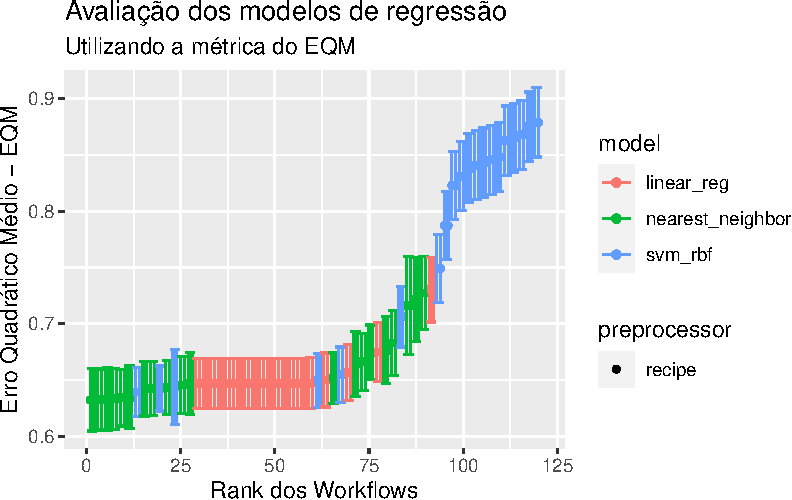
\includegraphics{tufte_svm_regressao_files/figure-pdf/unnamed-chunk-17-1.pdf}

}

\end{figure}

Perceba que no gráfico acima, temos os 8 modelos avaliados no
\(8\)-\emph{folds cross-validation}. Portanto, para cada um dos modelos
comparados, temos 8 avaliações. Caso deseje avaliar as métricas do
melhor cenário de cada um dos modelos, fazemos:

\begin{Shaded}
\begin{Highlighting}[]
\InformationTok{\textasciigrave{}\textasciigrave{}\textasciigrave{}\{r\}}
\NormalTok{melhores }\OtherTok{\textless{}{-}} 
\NormalTok{  treino }\SpecialCharTok{|\textgreater{}} 
  \FunctionTok{rank\_results}\NormalTok{(}\AttributeTok{select\_best =} \ConstantTok{TRUE}\NormalTok{, }\AttributeTok{rank\_metric =} \StringTok{"rmse"}\NormalTok{)}

\FunctionTok{autoplot}\NormalTok{(treino, }\AttributeTok{select\_best =} \ConstantTok{TRUE}\NormalTok{)}
\InformationTok{\textasciigrave{}\textasciigrave{}\textasciigrave{}}
\end{Highlighting}
\end{Shaded}

\begin{figure}[H]

{\centering 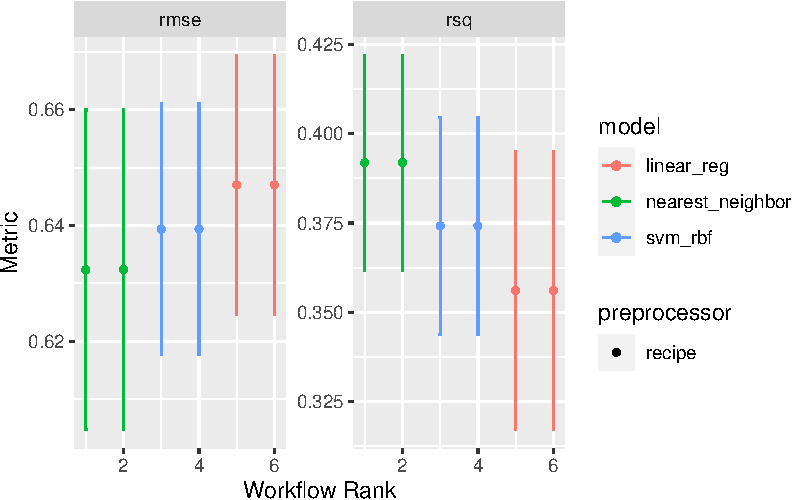
\includegraphics{tufte_svm_regressao_files/figure-pdf/unnamed-chunk-18-1.pdf}

}

\end{figure}

Vamos agora selecionar o melhor modelo dentre os modelos comparados.
Isso não quer dizer que o modelo seja bom para resolver o problema em
questão. Para ver um rank e saber qual modelo e receita foram as
melhores, fazemos:

\begin{Shaded}
\begin{Highlighting}[]
\InformationTok{\textasciigrave{}\textasciigrave{}\textasciigrave{}\{r\}}
\NormalTok{treino }\SpecialCharTok{|\textgreater{}} 
  \FunctionTok{rank\_results}\NormalTok{()}
\InformationTok{\textasciigrave{}\textasciigrave{}\textasciigrave{}}
\end{Highlighting}
\end{Shaded}

\begin{verbatim}
# A tibble: 240 x 9
   wflow_id         .config .metric  mean std_err     n preprocessor model  rank
   <chr>            <chr>   <chr>   <dbl>   <dbl> <int> <chr>        <chr> <int>
 1 recipe_2_knn_fit Prepro~ rmse    0.632  0.0168     8 recipe       near~     1
 2 recipe_2_knn_fit Prepro~ rsq     0.392  0.0182     8 recipe       near~     1
 3 recipe_1_knn_fit Prepro~ rmse    0.632  0.0168     8 recipe       near~     2
 4 recipe_1_knn_fit Prepro~ rsq     0.392  0.0182     8 recipe       near~     2
 5 recipe_1_knn_fit Prepro~ rmse    0.633  0.0165     8 recipe       near~     3
 6 recipe_1_knn_fit Prepro~ rsq     0.391  0.0174     8 recipe       near~     3
 7 recipe_2_knn_fit Prepro~ rmse    0.633  0.0165     8 recipe       near~     4
 8 recipe_2_knn_fit Prepro~ rsq     0.391  0.0174     8 recipe       near~     4
 9 recipe_2_knn_fit Prepro~ rmse    0.633  0.0169     8 recipe       near~     5
10 recipe_2_knn_fit Prepro~ rsq     0.390  0.0188     8 recipe       near~     5
# i 230 more rows
\end{verbatim}

Assim, podemos perceber que a \texttt{receita\_1} combinada com o modelo
\(k\)NN é o melhor escolha entre os modelos e receitas comparadas.
Portanto:

\begin{Shaded}
\begin{Highlighting}[]
\InformationTok{\textasciigrave{}\textasciigrave{}\textasciigrave{}\{r\}}
\NormalTok{melhor\_modelo }\OtherTok{\textless{}{-}} 
\NormalTok{  treino }\SpecialCharTok{|\textgreater{}} 
  \FunctionTok{extract\_workflow\_set\_result}\NormalTok{(}\AttributeTok{id =} \StringTok{"recipe\_1\_knn\_fit"}\NormalTok{) }\SpecialCharTok{|\textgreater{}} 
  \FunctionTok{select\_best}\NormalTok{(}\AttributeTok{metric =} \StringTok{"rmse"}\NormalTok{)}

\NormalTok{melhor\_modelo}
\InformationTok{\textasciigrave{}\textasciigrave{}\textasciigrave{}}
\end{Highlighting}
\end{Shaded}

\begin{verbatim}
# A tibble: 1 x 3
  neighbors dist_power .config              
      <int>      <dbl> <chr>                
1        12       1.47 Preprocessor1_Model15
\end{verbatim}

\hypertarget{avaliauxe7uxe3o-final-do-melhor-modelo}{%
\subsubsection{Avaliação final do melhor
modelo}\label{avaliauxe7uxe3o-final-do-melhor-modelo}}

Após a escolha do melhor modelo e da estimação de seus hiperparâmetros,
nesse caso, o modelo \(k\)NN com \(k = 12\) e
\texttt{dist\_power\ \textbackslash{}approx\ 1.47}, precisamos testar o
desempenho do modelo final segundo a base de dados de teste. Para tanto,
utilizamos a função \texttt{last\_fit} do pacote
\href{https://tune.tidymodels.org/reference/last_fit.html}{tune}. Temos
que:

\begin{Shaded}
\begin{Highlighting}[]
\InformationTok{\textasciigrave{}\textasciigrave{}\textasciigrave{}\{r\}}
\NormalTok{wf\_final }\OtherTok{\textless{}{-}} 
\NormalTok{  treino }\SpecialCharTok{|\textgreater{}} 
  \FunctionTok{extract\_workflow}\NormalTok{(}\AttributeTok{id =} \StringTok{"recipe\_1\_knn\_fit"}\NormalTok{) }\SpecialCharTok{|\textgreater{}} 
  \FunctionTok{finalize\_workflow}\NormalTok{(melhor\_modelo)}

\NormalTok{teste }\OtherTok{\textless{}{-}} 
\NormalTok{  wf\_final }\SpecialCharTok{|\textgreater{}} 
  \FunctionTok{last\_fit}\NormalTok{(}\AttributeTok{split =}\NormalTok{ divisao\_inicial)}

\NormalTok{teste}\SpecialCharTok{$}\NormalTok{.metrics}
\InformationTok{\textasciigrave{}\textasciigrave{}\textasciigrave{}}
\end{Highlighting}
\end{Shaded}

\begin{verbatim}
[[1]]
# A tibble: 2 x 4
  .metric .estimator .estimate .config             
  <chr>   <chr>          <dbl> <chr>               
1 rmse    standard       0.629 Preprocessor1_Model1
2 rsq     standard       0.405 Preprocessor1_Model1
\end{verbatim}

Agora que temos os hiperparâmetros estimados e temos uma boa estimativa
do risco preditivo real do modelo final selecionado, poderemos preceder
com um ajuste final, com toda a base de dados (treinamento + teste).

\begin{Shaded}
\begin{Highlighting}[]
\InformationTok{\textasciigrave{}\textasciigrave{}\textasciigrave{}\{r\}}
\NormalTok{modelo\_final }\OtherTok{\textless{}{-}} 
\NormalTok{  wf\_final }\SpecialCharTok{|\textgreater{}} 
  \FunctionTok{fit}\NormalTok{(dados)}
\InformationTok{\textasciigrave{}\textasciigrave{}\textasciigrave{}}
\end{Highlighting}
\end{Shaded}




\end{document}
